\documentclass[acmtog,screen,review,nonacm]{acmart}

\citestyle{acmauthoryear}

\makeatletter
\let\@authorsaddresses\@empty
\makeatother

\begin{document}



\author{Jilian Lubrat - 24374163}
\email{lubratj@tcd.ie}
\affiliation{%
  \institution{Trinity College}
  \city{Dublin}
  \country{Ireland}
}

\title{Computer Graphics Project}
\maketitle

\vspace*{0.1cm}
\section{\underline{Introduction}}
This report presents the work done on a computer graphics project entitled \textbf{ Toward a Futuristic Emerald Isle}. With this title, my idea was to create an emerald isle (in the literal meaning) in the sky, with a futurist society developed on it. I had several instructions for this project:
\begin{itemize}
  \item A minimum frame rate of 15fps when the application runs on the latest generation of CPUs.
  \item A controllable camera to move around the scene.
  \item Demonstration of an infinite scene: when the camera moves, the application should simulate an endingless effect.
  \item Implementation of one advanced feature chosen in a list of 9 features.
\end{itemize}
You can find the codebase of the application on GitHub : \url{https://github.com/LubratJilian/project_computer_graphic}.
\\
According to these instructions, I implemented a camera as the one we can find in First Player Shooter (FPS) games. From the list of advanced features I initially chose to implement the Real-time global illumination by voxel cone tracing. But after successfully voxelizing the space, I did not achieve the cone tracing implementation. After this, more precisely at the end of the project, I chose to implement  instancing to place trees and streetlamps in the city without altering a lot the fps. We will discuss this in more detail in the next section. In addition to that, because the scene takes place in the sky, I implemented a cloud generator, which creates clouds using Perlin Noise and moves the clouds as the camera moves. I also implemented a Phong Illumination Model and added material attribute to the objects to adapt their shading and diffusion. I reused the GLTF file importation for animations from Lab4. And I used an OBJ file loader found on the web (see the source in the last part), which I modified a little bit to adapt it.
\\

\section{\underline{Historic of the project}}
I took five screenshots of the rendering throughout the development. We will retrace the implementation of the project through these  screenshots. 
\\

First, I used the base code from Lab2 with the skybox. Thanks to that, I implement the SkyBox class and created the shaders for it. I searched a texture for my skybox, but I wanted something simple, as if I were above the clouds in an airplane, so I chose to just use color for my SkyBox. To implement the idea of the scene being endingless, I fixed the center of the skybox to my camera, which allows me to move around without going out of the scene.\\
I implemented a class for the camera, similar to the one we can found in some video games. We move with WASD and can turn around with the mouse. After that, I started to model an isle with emerald crystals I found on the web. I modeled a base covered by crystals, and the texture was blue, so I modified it with a Python script and changed it to something more green.\\
I chose to export the isle with the OBJ extension because the GLTF loader did not work well when I export from Blender in GLTF. Something was wrong with the export parameters, but I did not know what. I found an OBJ file loader in a tutorial on the web, so I decided to use it to import my isle. And I then created a class Object with the shaders to import my isle. With all of this, I obtained the render we can see on Fig \ref{fig:Fig 1}.
\begin{figure}[H]
    \centering
    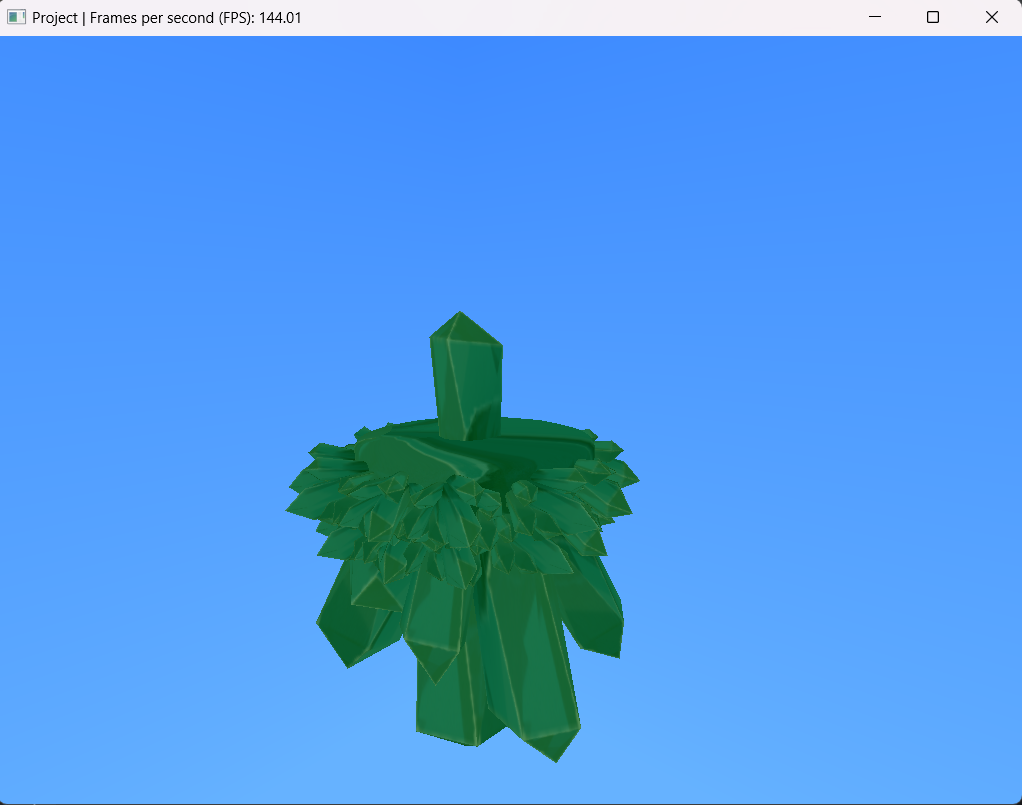
\includegraphics[width=0.5\linewidth]{save/Save1_27_11_2024.png}
    \caption{First Screenshot}
    \label{fig:Fig 1}
\end{figure}

Secondly, I started thinking about the lighting and wanted to implement global illumination. To do that, I chose to try voxel cone tracing. I started by implementing the voxelization of the scene. I chose to stay with Opengl 3.3, so I learned how to deal with array of textures, which are useful for saving the voxelized scene as different layers of the rendered scene. After successfully voxelizing the scene, I tried to implement the cone tracing, which is easy in theory but more complex in practice. I did not know how to transition from theory to practice. I searched on the web,  but most resources were for newer version of OpenGl or did not work in my project. So, I chose to implement a Phong illumination with shadows.\\
I started by implementing two classes: Light and Lights. The first class implements the light itself and the second stores all the lights and shadows. With three lights (blue, red and green), I obtained the render shown in Fig \ref{fig:Fig 2}. At this point, I did not have Phong illumination just the three lights influencing the color of the isle.\\
I added the Bot class to load GLTF files and animations, reusing the animation from Lab4. I implemented the shaders linked to the Bot class but have not yet accounted for the impact of the lights.

\begin{figure}[H]
    \centering
    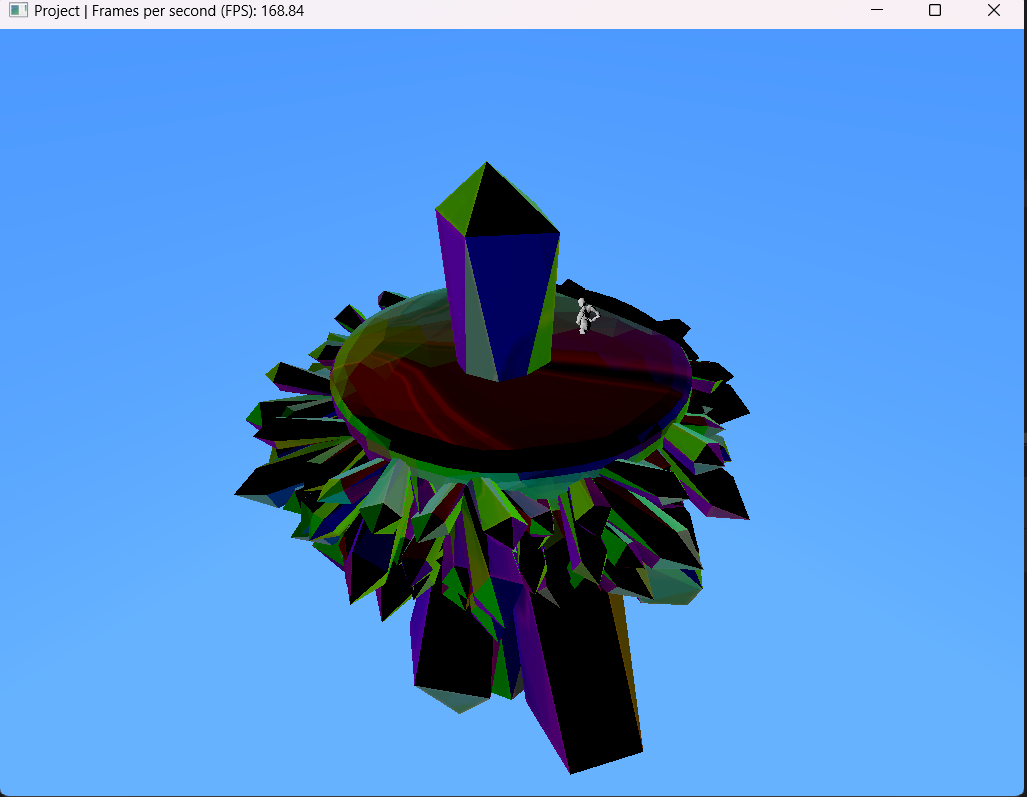
\includegraphics[width=0.5\linewidth]{save/Save2_08_12_2024.png}
    \caption{Second Screenshot}
    \label{fig:Fig 2}
\end{figure}

Thirdly, I continued the implementation of the Phong illumination. For this, I reused what I learned with texture arrays to store the shadows from each light and added the shadows to the fragment shader of the isle. With two lamps, one red and one green on each side, we obtained the result shown in Fig \ref{fig:Fig 3}, where we can see the shadows of the large crystal in the center, depending to each lights.

\begin{figure}[H]
    \centering
    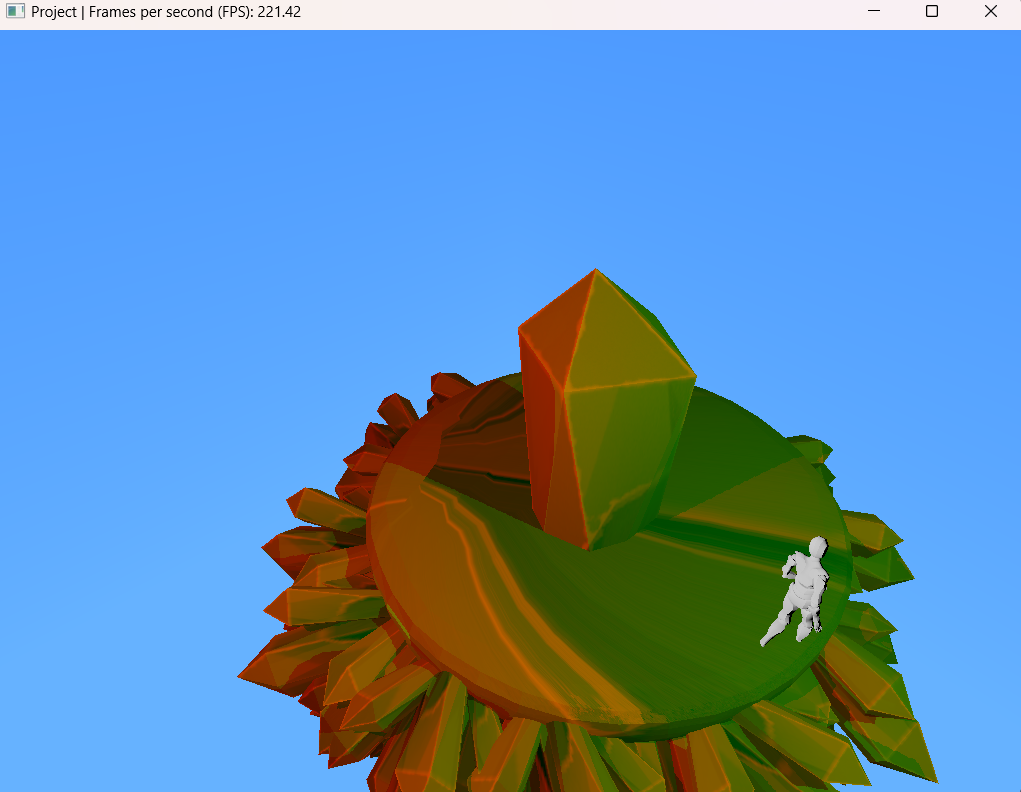
\includegraphics[width=0.5\linewidth]{save/Save3_09_12_2024.png}
    \caption{Third Screenshot}
    \label{fig:Fig 3}
\end{figure}

Fourth, I found the endingless scene effect to be not very convincing because when the isle disappears, it feels like we are like trapped in the sky. I came up with the idea to add clouds to simulate the the movement of the camera, even when the isle is too far. To do this, I added a CloudsGenerator class, which creates ten layers of Perlin Noise and renders them in superposition to give the effect of clouds. Thanks to this, when the camera moves, even if it is far from the island, we have the sensation of movement. \\
In addition, I found some futuristic buildings on the web and I placed them on Blender, then exported them as an OBJ file. I also added the ability to use color when rendering objects, because before that, only textures could be used for rendering. In addition, I created a road in Blender as well.
\\
 To finish, I added a StreetLamps class with a NetworkLoader class. The first one stores the StreetLamp object and it different positions to render it at the good location. The second one is used to load the position and the orientation of each streetlamps. The orientation is stored as a color of the vertices that represent the position. 
 \\
 In the first version, all the streetlamps were different objects and rendered independently. However, implementing an advanced feature was still required, so I chose to implement the instancing. In fact, this is what I did  for the streetlamps, so I modified the class to add instancing and improve performance at the same time.  With all of this we obtain the render, we can see in Fig \ref{fig:Fig 4} 

\begin{figure}[H]
    \centering
    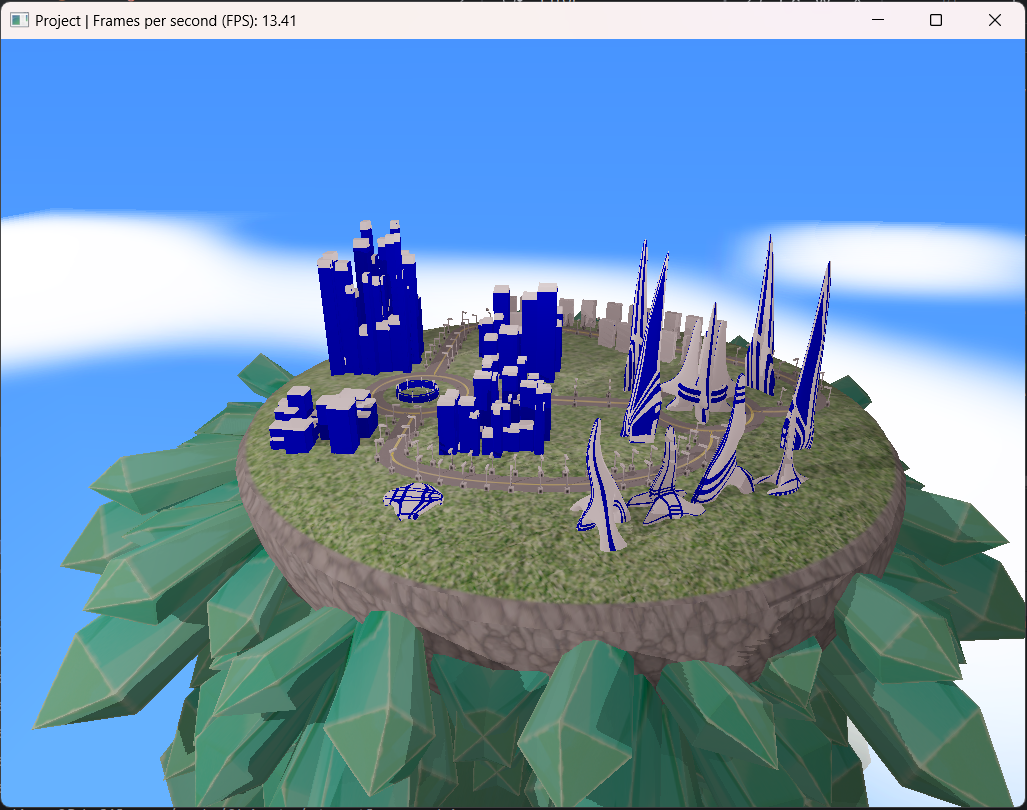
\includegraphics[width=0.5\linewidth]{save/Save4_24_12_2024.png}
    \caption{Fourth Screenshot}
    \label{fig:Fig 4}
\end{figure}

Fifthly, to finish the project, I added some trees with the StreetLamps and NetworkLoader implementation. I updated the Streetlamps class to take an object as input rather than just rendering streetlamps. 
\\
To finish the project, I had to add some animations and place them on the isle. I tried to create new animations in Blender with the bot from lab 4 and some HVD filse. Everything was working on Blender, but after exporting, the bot was moving without animation. I tried all the export parameters, but I never found the correct one. After that, I decided to change my approach and just add several bots running like, as in Lab4. I planned to use the two previously created classes. I modified the implementation to pass either an object or a bot, and according to that, the class would handle the appropriate operations. But, I encountered a bug when trying to render more than one bot: the skin of the bot is missing, and only the joints were rendered. To finish, I kept only one bot and rendered it in red to better view it. The render is shown in Fig \ref{fig:Fig 5}.

\begin{figure}[H]
    \centering
    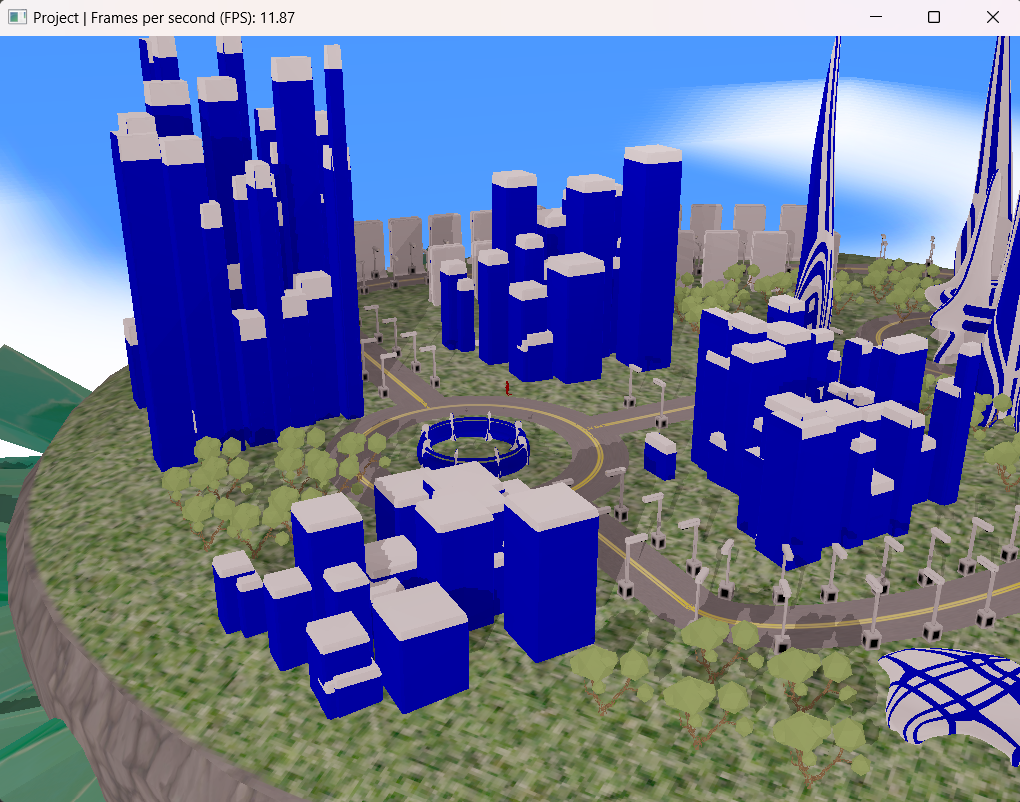
\includegraphics[width=0.5\linewidth]{save/Save5_25_12_2024.png}
    \caption{Fifth Screenshot}
    \label{fig:Fig 5}
\end{figure}

\section{\underline{Quality and Robustness}}
The project is highly modular, thanks to the implementation of each feature in different classes. It is easy to change some parts without altering all the code. In addition, there are shaders for each class, so if we need to change the way something is rendered, we can simply modify its shaders. In addition, to adapt the project to different materials, the quality of the shadows and of the clouds can be easily modified. 
\\
\section{\underline{Limitation and Future work}}
The project is limited by several factors. 
\\
Firstly, the size of the SkyBox is too large. I did this to respect the rule of endingless of the scene, as I did not want the isle to clip into the SkyBox. However, rendering clouds of this size is very expensive.\\
Secondly, there is a problem with the bot that prevents rendering more than one at the same time. \\
Thirdly, how the separation between the isle and the camera is implemented, because it is done by scaling smaller the isle according to the distance. It gives the impression of high speed when the distance increases, which feels strange.
\\\\
To improve the project, the first thing to do would be to fix the rendering issue the bots and add texture management.
\\
The second improvement would be to change the way the SkyBox is rendered. For example, we could load a texture representing the view from the camera with a larger field of view on each side, which would allow us to reduce the size of the SkyBox. With a sufficiently large field of view, even if the isle is outside the SkyBox, it would still be represented on the texture, which could be placed on a side of the SkyBox.\\
The last improvement would be to modify how the isle is scaled when the camera moves away from it.
\\
\section{\underline{Conclusion}}
To conclude, this project was a great way to implement and improve everything we covered in computer graphics during the semester, and to learn some new things, such as how to manage a large number of textures. It allowed me to apply theoretical concepts to a real project. Despite the challenges, such as optimizing performance and fixing bugs, I gained valuable experience that will be useful for future projects. Looking back, I feel more confident in handling complex graphical systems and look forward to exploring more advanced techniques in the future.
\\
\section{\underline{Acknowledgment}}
Code of the OBJ loader : \url{https://github.com/huamulan/OpenGL-tutorial/blob/master/common/objloader.cpp} found on the website opengl-tutorial.org (\url{www.opengl-tutorial.org}).
\\

Models sources :
\begin{itemize}
    \item Buildings: \url{https://sketchfab.com/3d-models/bionic-architecture-6a40bae62e614e0990742871eed788f6} by Vishchun (\url{https://sketchfab.com/vishchun}), licensed under CC-BY-4.0 \url{http://creativecommons.org/licenses/by/4.0/}
    \item Street Lamps: \url{https://sketchfab.com/3d-models/low-poly-light-street-32bd9bc6f27844e795bd5030091cf96e} by xboyghost07 (\url{https://sketchfab.com/xboyghost07}), licensed under CC-BY-4.0 \url{http://creativecommons.org/licenses/by/4.0/}
    \item Crytals: \url{https://sketchfab.com/3d-models/low-poly-crystals-4a6320d8c4d243eebfe6b83e67511073} by elliothunter72 (\url{https://sketchfab.com/elliothunter72}), licensed under CC-BY-4.0 \url{http://creativecommons.org/licenses/by/4.0/}
    \item Tree: \url{https://free3d.com/fr/3d-model/low_poly_tree-816203.html} by Kiprus (\url{https://free3d.com/fr/user/kiprus})
\end{itemize}

Textures sources :
\begin{itemize}
    \item Road texture: \url{https://www.freepik.com/free-photo/lines-traffic-paved-roads-background_3738056.htm#fromView=search&page=2&position=45&\allowbreak/uuid=622c369a-e8fc-4e3c-b1a8-b82a6f177413} by Jcomp (\url{https://www.freepik.com/author/jcomp})
    \item Grass texture: \url{https://www.freepik.com/free-photo/green-fake-grass-background_2791853.htm#fromView=keyword&page=1&position=1&uuid=a285431a-f409-4749-b93d-\allowbreak7c2e118cd356} by Rawpixel.com (\url{https://www.freepik.com/author/rawpixel-com})
    \item Stone texture: \url{https://fr.pinterest.com/pin/yay-rock-texture-by-aecoleman-avery-coleman-cghub--547961479634286861/} by Aecoleman (\url{https://fr.pinterest.com/refugee3d/}
    \item Crystals texture: Same as Crystals model, \url{https://sketchfab.com/3d-models/low-poly-\allowbreakcrystals-4a6320d8c4d243eebfe6b83e67511073} by elliothunter72 (\url{https://sketchfab.com/elliothunter72}), \\licensed under CC-BY-4.0 \url{http://creativecommons.org/licenses/by/4.0/}
\end{itemize}
\end{document}
